\documentclass{article}

\usepackage{graphicx}
\usepackage{tikz}
\usepackage{tikzsymbols}
\usetikzlibrary{calc,patterns,shapes.geometric}
\pagestyle{empty}
\usepackage[margin=0pt]{geometry}
\geometry{papersize={14in,12in}}

\def\centerarc[#1](#2)(#3:#4:#5){\draw[#1] ($(#2)+({#5*cos(#3)},{#5*sin(#3)})$) arc (#3:#4:#5);}

\begin{document}
	\begin{figure}
		\centering
		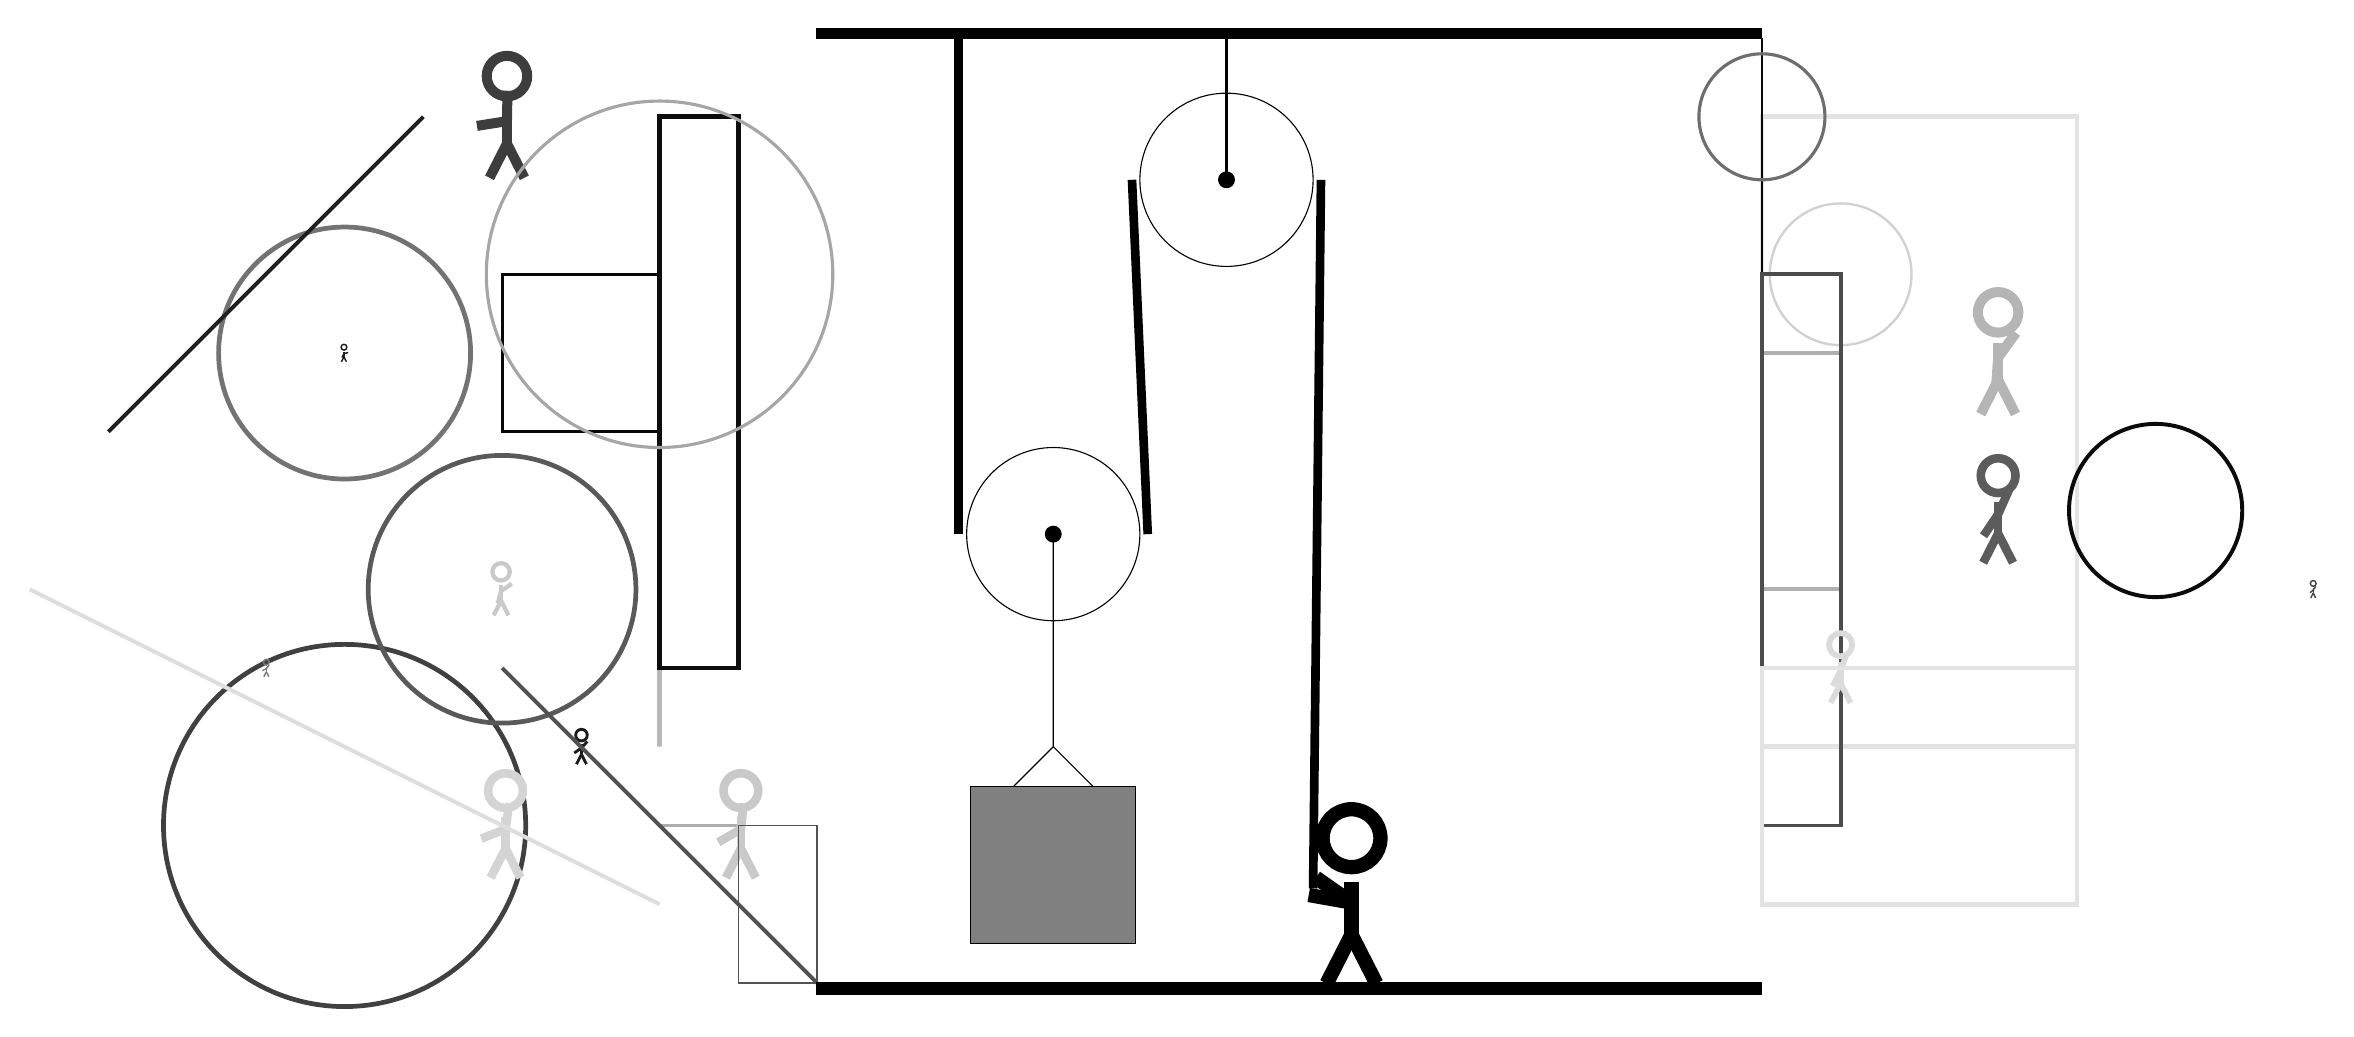
\begin{tikzpicture}
			%%%%% START %%%%%
			
			\draw[fill=black] (-2, 9) rectangle (10, 9.125);
			
			\draw (3.2, 7.2) circle (1.1);
			\draw[fill=black] (3.2, 7.2) circle (0.1);
			\draw[thick] (3.2, 7.2) -- (3.2, 9);
			
			\draw (1, 2.7) circle (1.1);
			\draw[fill=black] (1, 2.7) circle (0.1);
			
			\draw (1, 2.7) -- (1, 0) -- (0.5, -0.5);
			\draw (1, 0) -- (1.5, -0.5);
			\draw[fill=black!50] (-0.05, -0.5) rectangle (2.05, -2.5);
			
			\draw[line width=0.5mm, color=black!32](-3, -1) -- (-4, -1);
			
			\node[line width=0.7mm, color=black!73] at (17, 2) {\Strichmaxerl[1][43][53]};
			\draw [line width=0.6mm, color=black!75](-8, -1) circle (2.3);
			\draw [line width=0.3mm, color=black!18](11, 6) circle (0.9);
			\draw[line width=0.5mm, color=black!31] (10, 5) rectangle (11, 2);
			\node[line width=0.5mm, color=black!21] at (-3, -1) {\Strichmaxerl[6][30][84]};
			\draw[line width=0.4mm, color=black!97] (-4, 4) rectangle (-6, 6);
			\node[line width=0.3mm, color=black!89] at (-5, 0) {\Strichmaxerl[2][35][48]};
			\draw[line width=0.7mm, color=black!28] (-4, 1) rectangle (-4, 0);
			\draw [line width=0.6mm, color=black!65](-6, 2) circle (1.7);
			\node[line width=0.3mm, color=black!29] at (13, 5) {\Strichmaxerl[7][86][54]};
			
			\draw[line width=0.6mm, color=black!11] (10, 8) rectangle (14, 0);
			\draw [line width=0.5mm, color=black!96](15, 3) circle (1.1);
			\draw[line width=0.2mm, color=black!97] (10, 9) rectangle (10, 3);
			\draw[line width=0.6mm, color=black!95] (-4, 8) rectangle (-3, 1);
			\node[line width=0.7mm, color=black!76] at (-6, 8) {\Strichmaxerl[7][9][89]};
			
			\draw[line width=0.5mm, color=black!70] (11, -1) rectangle (10, 6);
			
			\node[line width=0.5mm, color=black!89] at (-8, 5) {\Strichmaxerl[1][62][15]};
			\draw [line width=0.4mm, color=black!57](10, 8) circle (0.8);
			\draw [line width=0.4mm, color=black!35](-4, 6) circle (2.2);
			\node[line width=0.2mm, color=black!17] at (-6, -1) {\Strichmaxerl[6][21][82]};
			\node[line width=0.7mm, color=black!64] at (13, 3) {\Strichmaxerl[6][56][66]};
			\node[line width=0.5mm, color=black!52] at (-9, 1) {\Strichmaxerl[1][27][50]};
			\node[line width=0.4mm, color=black!14] at (11, 1) {\Strichmaxerl[4][63][70]};
			\draw[line width=0.6mm, color=black!11] (10, -2) rectangle (14, 1);
			
			\draw[line width=0.5mm, color=black!68](-2, -3) -- (-6, 1);
			\draw [line width=0.6mm, color=black!55](-8, 5) circle (1.6);
			\draw[line width=0.5mm, color=black!88](-7, 8) -- (-11, 4);
			\draw[line width=0.2mm, color=black!68] (-3, -1) rectangle (-2, -3);
			\node[line width=0.6mm, color=black!21] at (-6, 2) {\Strichmaxerl[3][75][35]};
			\draw[line width=0.5mm, color=black!13](-4, -2) -- (-12, 2);
			
			\draw[line width=1.1mm] (-0.2, 9) -- (-0.2, 2.7);
			\centerarc[line width=1.1mm](1, 2.7)(180:360:1.2000000000000002);
			\draw[line width=1.1mm](2.2, 2.7) -- (2.0, 7.2);
			\centerarc[line width=1.1mm](3.2, 7.2)(0:180:1.2000000000000002);
			\draw[line width=1.1mm](4.4, 7.2) -- (4.3, -1.8);
			
			\node at (4.7, -1.9) {\Strichmaxerl[10][-35][170]};
			
			\draw[fill=black] (-2, -3) rectangle (10, -3.15);
			
			%%%%% END %%%%%
		\end{tikzpicture}
	\end{figure}	
\end{document}